\chapter{Analiza wyników}

Posiadając już dane na temat zależności siły w czasie dla różnych prędkości rozciągania można było przystąpić do analizy wyników.

\section{Znajdowanie siły rozplatania}

Pierwszym etapem był wybór z zestawu danych maksymalnej siły rozplatania. Metoda najprostsza, czyli branie jako siły rozplatania maksymalnej siły z surowych wykresów siły od rozciągnięcia ma te zalety, że jest proste i najmniej czasochłonne, niestety wynik ten byłby zakłamany w wyniku drgań termicznych, które powodują powstawanie znacznych szumów na wykresie siły od rozciągnięcia. W celu eliminacji tego niepożądanego zjawiska zastosowano wygładzanie.

Aby uzyskać wygładzone krzywe napisano skrypt w języku Python (smooth.py) w wersji 2.6.5 na systemie Ubuntu 10.04 w wersji serwerowej. Skrypt ten odpowiedzialny był za wygładzanie wykresów metodą średniej kroczącej Gaussa z zadaną szerokością ramki. Jego główną część stanowi algorytm opisany na stronie \cite{gauss}. 

Zasada jego działania polega na pobraniu liczby punktów odpowiadających szerokości ramki wokół danego punktu na wykresie niewygładzonym, a następnie wyliczeniu średniej ważonej, gdzie wagi odpowiadają rozkładowi Gaussa dla liczby punktów odpowiadających szerokości ramki.

Szerokość ramki użyta w publikacji \cite{1tki} wynosiła 0.16 nm i została użyta również w tym przypadku. Przy wygładzaniu należało uwzględnić fakt, że używana stała szerokość w nm odpowiadała różnej liczbie punktów na wykresie. Znając szybkość rozciągania oraz krok zapisu danych obliczenie liczby potrzebnych punktów stało się trywialne.

\begin{center}
\begin{figure}[h]
\begin{centering}
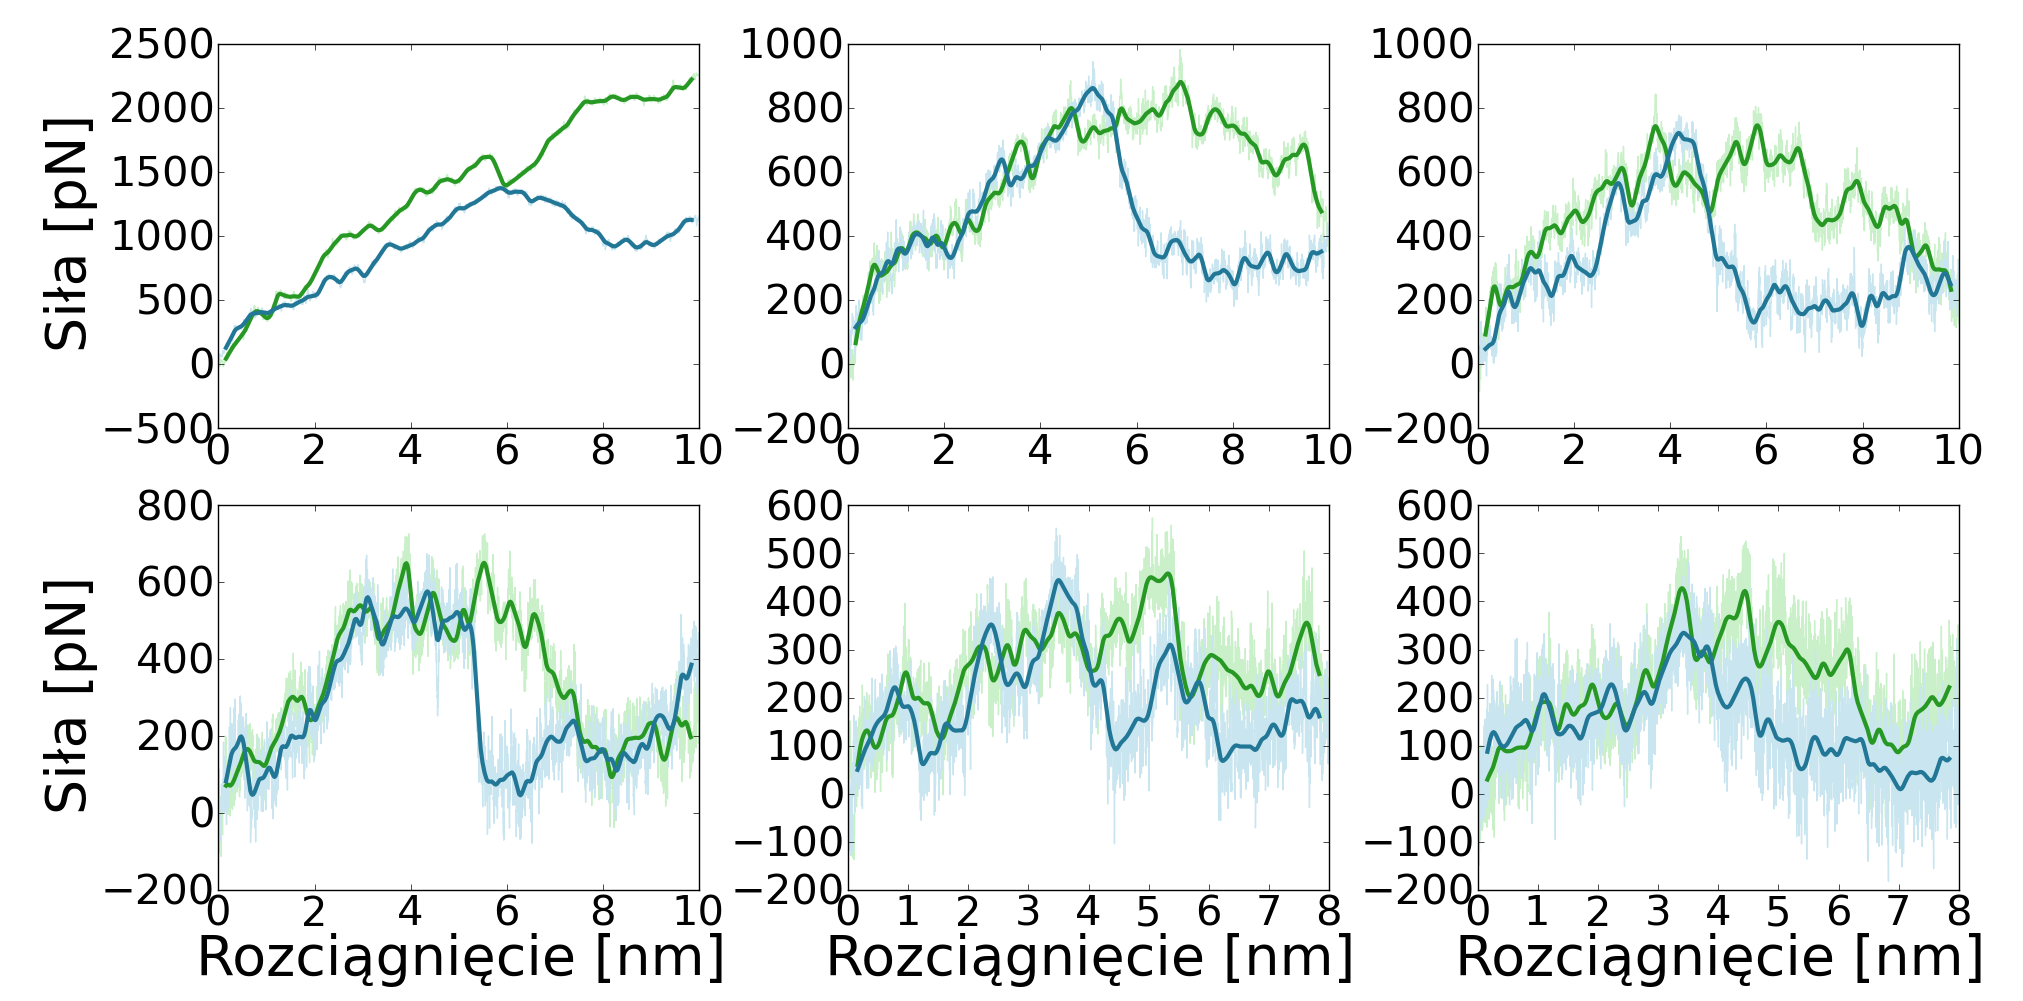
\includegraphics[width=150mm]{./rys/smooth.png}
\caption{Wygładzone krzywe zależności siły od rozciągnięcia dla 6 prędkości rozciągania dla końców białka.}
\end{centering}
\end{figure}

\end{center}

Posiadając już wygładzone wykresy siły od rozciągnięcia jako siły rozplatania bierze się maksymalne siły na wygładzonym wykresie siły od rozciągnięcia. Dla porównania z wynikami literaturowymi odczytano siły rozplatania z wykresu w publikacji \cite{1tki}.

\begin{center}
\begin{table}[h]
\centering
  \begin{tabular}{| r | c | c | c | c |}
  \hline
      & \multicolumn{4}{|c|}{Maksymalna siła [pN]} \\
\cline{2-5}
	Prędkość & \multicolumn{2}{|c|}{Z symulacji} & \multicolumn{2}{|c|}{Z publikacji} \\
\cline{2-5}
[nm/ns] &  N-koniec  & C-koniec &  N-koniec  & C-koniec \\
  \hline
  50 & 1372 & 1618  & 1323 & 1376\\
  10 & 815 & 822 & 796 & 710 \\
  5 &  720 & 745 & 645 & 526 \\
  2 & 576 & 650 &  366 & 559\\
  0.8 & 443 & 459 &  495 & 667\\
  0.4 & 334 & 429 & 452 & 538\\
  \hline
  \end{tabular}
  \caption{Maksymalne siły rozplatania dla różnych prędkości rozciągania dla symulacji oraz z danych literaturowych.}
\end{table}
\end{center}

\section{Dopasowanie krzywej teoretycznej do wyników}

\subsection{Mechanizm postępowania}

Korzystając z modelu teoretycznego Hummera--Szabo omówionego we wstępie na podstawie publikacji \cite{Hummer_Szabo_2003} oraz metodologii prezentowanej w publikacji \cite{szul} napisano skrypt w środowisku programistycznym Python, który miał za zadanie poprzez optymalizację parametrów kinetycznych znaleźć jak najlepsze dopasowanie krzywej teoretycznej dla otrzymanych wyników.

Do obliczenia teoretycznej zależności średniej siły rozplatania od prędkości rozciągania służy wzór \ref{eq:wyn} przedstawiony we wprowadzeniu.

Do optymalizacji parametrów $\mathbf{p}=\left\lbrace k_0, x_b, \kappa_m\right\rbrace$ służy funkcja najmniejszych kwadratów $S(\mathbf{p})$:

\[
S(\mathbf{p})=\sum_{i=1}^n r_i^2 
\]
\[
r_i=F_{s, i} - \overline{F}(v_i, \mathbf{p})
\]

Gdzie $F_{s,i}$ oznacza $i$-tą siłę rozplatana wziętą z symulacji dla prędkości $v_i$, a $\overline{F}(v_i, \mathbf{p})$ oznacza teoretyczną wartość siły obliczoną dla $i$-tej prędkości i parametrów $\mathbf{p}$.

Mając tak zdefiniowaną funkcję najmniejszych kwadratów minimalizuje się ją wewnętrzną funkcją \texttt{fmin()} pakietu SciPy \cite{Scipy} języka Python ze względu na parametry $\mathbf{p}$. Jest to optymalizacja metodą Simplex. Wbudowana w Pythona metoda najmniejszych kwadratów jest szybciej zbieżna niż optymalizacja metodą Simplex, jednak przy znacznej różnicy parametrów początkowych od optymalnych parametrów powoduje powstawanie błędów. Kod minimalizowanej funkcji błędu przedstawiony jest w \ref{kod:err} .
%\linespread{1}
\begin{lstlisting}[label={kod:err}, caption={Minimalizowana funkcja błędu.}]
def err(p_l):
	out=0
	fs=F(p_l,V)
	out=((fs - f)**2).sum()
	return out
p1=fmin(err, p, xtol=1e-5, maxiter=1000000, maxfun=1000000)
\end{lstlisting}

Funkcja ta pobiera parametry do optymalizacji jako lokalne \texttt{p\_l}. Na ich podstawie oraz na podstawie prędkości \texttt{V} liczona jest teoretyczna wartość siły \texttt{fs}. Suma kwadratów różnic siły teoretycznej \texttt{fs} oraz globalnej wartości siły \texttt{f} obliczana jest w linii nr 4. Do uzyskania wartości teoretycznych użyta jest funkcja \texttt{F()}, która zdefiniowana jest następująco:

\begin{lstlisting}[label={kod:F}, caption={Znajdowanie wartości funkcji teoretycznej dla zadanych parametrów i prędkości.}]

s = lambda t, vel_l, p_l: exp(-p_l[0] * exp(-0.5*ks*p_l[1]**2)/(vel_l*ks*p_l[1]*(p_l[2]/(p_l[2]+ks))**(1.5))*(exp(ks*vel_l*p_l[1]*t - (0.5*(ks*vel_l*t)**2)/(ks+p_l[2]))-1))

def F(p_l, x_l):
	k0_l, xb_l, km_l = p_l[0], p_l[1], p_l[2]
	D_l=k0_l * sqrt(2*pi) / (km_l**(1.5)*xb_l*exp(-0.5*km_l*xb_l**2))
	b=D_l*(km_l+ks)
	out=[]
	for i in range(len(x_l)):
		vel_l = x_l [i]
		a=(xb_l*D_l*(km_l+ks)**2/(ks*vel_l)+1)
		tau=(lambertW(-exp(-a))+a)/b
		out.append(-ks*300*kb*(xb_l-vel_l*quad(s,0,tau, args=(vel_l, p_l), epsabs=1e-16)[0]))
	return array(out)
\end{lstlisting}

Wartości $\overline{F}(v_i, \mathbf{p})$ stanowiące wynik równania \ref{eq:wyn} obliczane są w linii nr 13. Równania tego nie da się rozwiązać analitycznie, przez co występująca w nim całka oznaczona liczona jest numerycznie. Całka ta liczona jest dla funkcji \texttt{s} zdefiniowanej w linii nr 1, która stanowi równocześnie bezpośrednie odzwierciedlenie funkcji \ref{eq:s_t} z wprowadzenia. Granice całkowania zdefiniowane są od \texttt{0} do \texttt{tau}, które znajdywane jest na podstawie równania \ref{eq:rozw_szczeg}. Równanie to nie może być rozwiązane analitycznie, ponieważ otrzymujemy równanie typu:

\begin{equation}
a=b\tau + e^{-b\tau}
\label{eq:omega}
\end{equation} 

Gdzie \texttt{a} i \texttt{b} zdefiniowane są w kodzie. Do rozwiązania tego równania użyta została funkcja $\Omega$ Lamberta, która zdefiniowana jest jako funkcja odwrotna do $W e^W$ \cite{lambert}. Rozwiązanie równania 5.1 znalezione zostało przy pomocy programu Wolfram Alpha\cite{wolfram} i przedstawione zostało w linii nr 12 kodu. Wartości funkcji Lamberta liczone są według procedury \texttt{lambertw()}, która została zaimportowana z pakietu SciPy w wersji 0.8\cite{Scipy}.

\subsection{Analiza metody dopasowania}

Mając maksymalne siły rozplatania z symulacji oraz dysponując danymi rozplatania w tych samych warunkach tej samej cząsteczki z publikacji \cite{1tki} oraz danymi eksperymentalnymi AFM z publikacji \cite{mechanoenz}, gdzie znaleziona średnia siła rozplatania dla 1TKI wyniosła około 50 pN dla prędkości 1 $\mu$m/s można przystąpić do analizy wyników. Odbywa się ona poprzez dopasowanie parametrów  $k_0$, $x_b$ i $\kappa_m$ do danych z symulacji oraz obliczenie na podstawie tych parametrów siły rozplatania dla prędkości 1 $\mu$m/s.

Zgodnie z teorią mikroskopową przedstawioną w publikacji \cite{Hummer_Szabo_2003} krzywa teoretyczna osiąga wartości ujemne poniżej prędkości równych iloczynowi $k_0$ i $x_b$, wobec czego jeśli $k_0 x_b > 1 \mu\text{m/s}$ odzyskanie siły rozplatania jest niemożliwe.

\begin{center}
\begin{figure}[h]
\begin{centering}
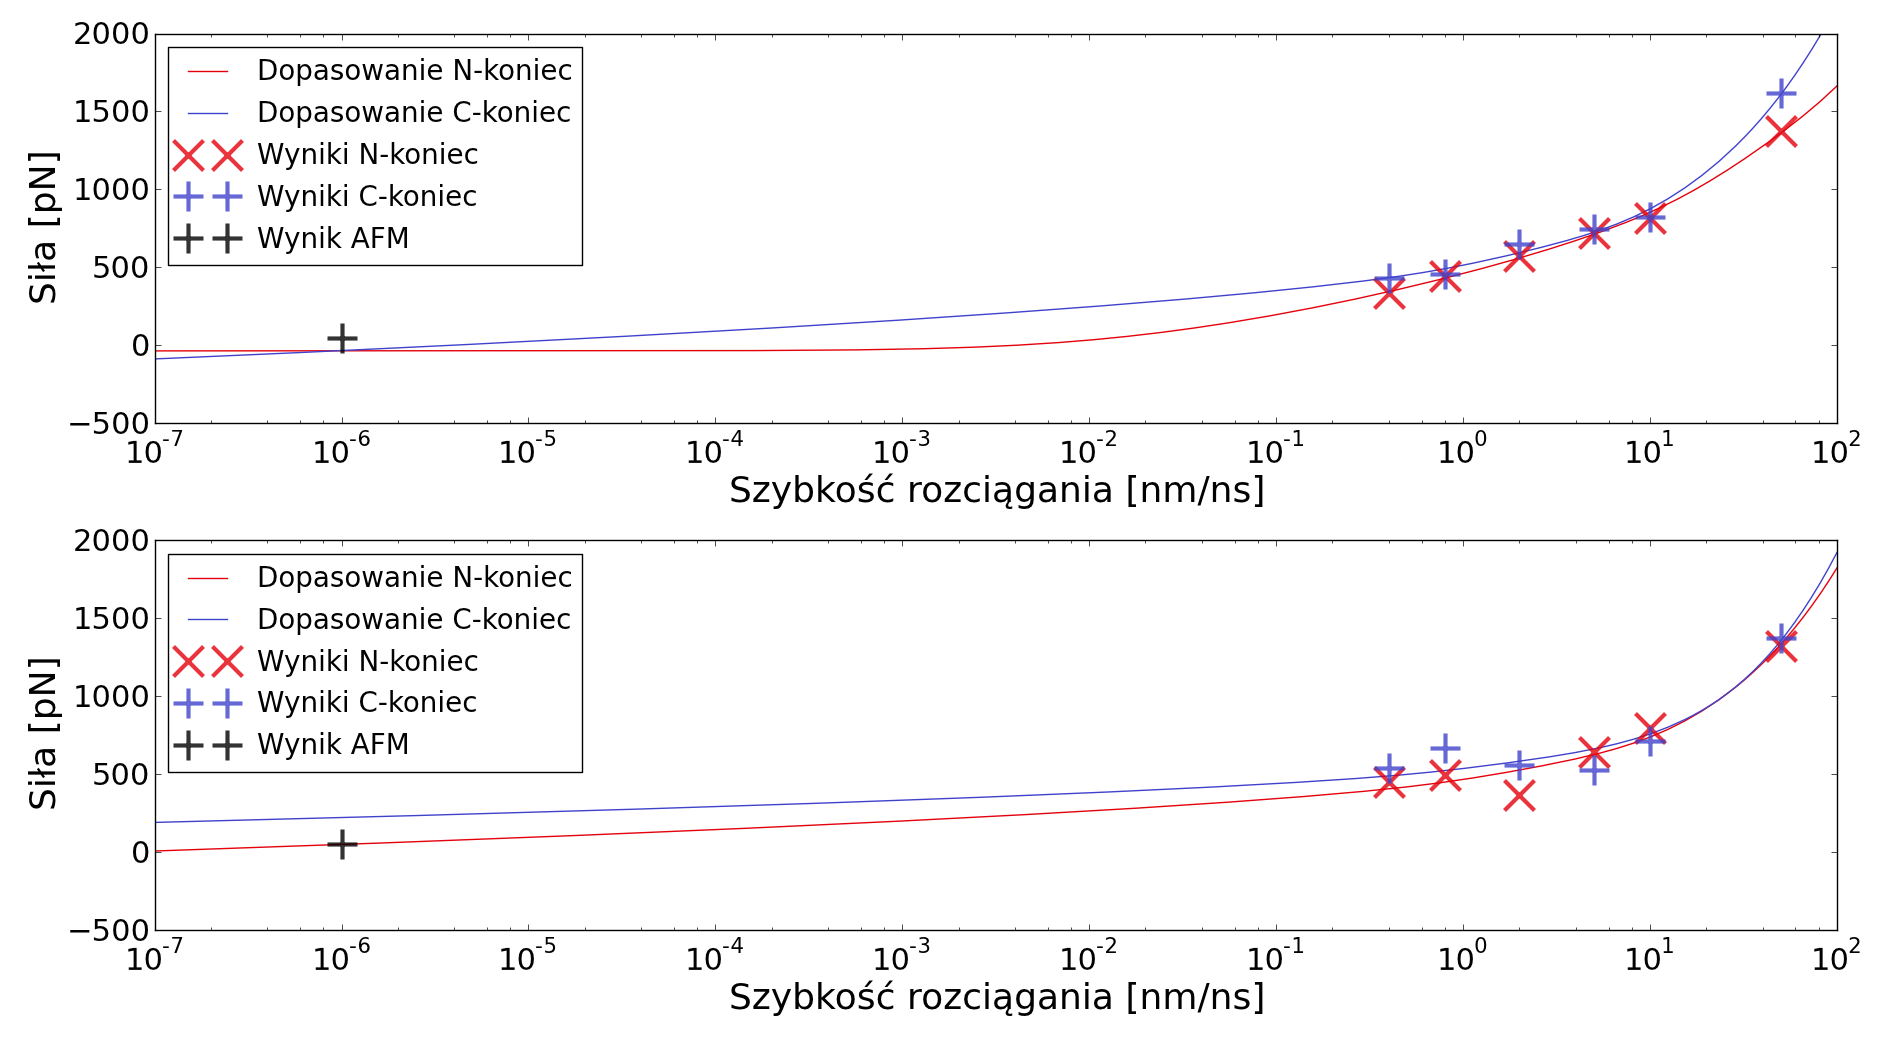
\includegraphics[width=150mm]{./rys/dop.png}
\caption{Wykresy siły rozplatania w zależności od szybkości rozciągania dla danych z symulacji (górny panel) oraz dla danych literaturowych (dolny panel) wraz z dopasowanymi krzywymi teoretycznymi.}
\end{centering}
\end{figure}
\end{center}

\begin{center}
\begin{table}[h]
\centering
  \begin{tabular}{ l l l l l}
  \hline
Koniec & $k_0$ [s$^{-1}$] & $x_b$ [nm] & $k_bT\kappa_m$ [N/m] & $x_b k_0$ [m/s] \\
  \hline
Symulacje \\
N & 7.944\e{7} & 0.04287& 38.36 & 3.41\e{-3} \\
C & 2.787\e{3} & 0.1960 & 3.669 & 4.56\e{-7} \\
\hline
Praca \cite{1tki}\\
N & 3.970\e{-1}& 0.347 & 1.804 & 1.38\e{-10} \\
C & 1.219\e{-26} & 1.101 & 0.5820 & 1.34\e{-35}\\
\hline
  \hline
  \end{tabular}
  \label{tab1}
  \caption{Parametry kinetyczne $k_0$, $x_b$ i $\kappa_m$ dla N i C-końca 1TKI z symulacji i z publikacji \cite{1tki}}
\end{table}
\end{center}

Z tabeli 5.2 wynika, że jedynie w przypadku parametrów odzyskanych z symulacji rozciągania dla N-końca dla publikacji \cite{1tki} sensowna jest próba odzyskania siły rozplatania dla prędkości 1$\mu$m/s. Dla tych parametrów wynosi ona 48.9 pN, co jest dość dobrym przybliżeniem wobec 50 pN eksperymentalnych. 

Zbadano również zależność uzyskiwanych parametrów kinetycznych od wyboru punktu startowego. Analizę tę wykonano dla danych pochodzących z symulacji dla C-końca.

\begin{center}
\begin{table}[h!]
\centering
  \begin{tabular}{ | l l l l l l l l l |}
  \hline
Parametr & & & & & & & & \\
\hline
$k_0$ 1.6$\times$ [s$^{-1}$] & 10$^{-17}$ \cellcolor{red}&10$^{-16}$ \cellcolor{green}& 10$^{-12}$ \cellcolor{green}& 10$^{-2}$ \cellcolor{green}& 10$^{2}$ \cellcolor{green}& 10$^{8}$ \cellcolor{green}& 10$^{10}$ \cellcolor{red} & 10$^{12}$ \cellcolor{red}\\
$x_b$ \e{-10}[m] & 0.5 \cellcolor{red}& 1 \cellcolor{green}& 2 \cellcolor{green}& 4 \cellcolor{green}& 6 \cellcolor{green}& 8 \cellcolor{green}& 10 \cellcolor{green}& 20 \cellcolor{red}\\
$\kappa_m$ \e{20} & 0.5\cellcolor{red} & 1\cellcolor{red} & 2 \cellcolor{green}& 3 \cellcolor{green}& 4 \cellcolor{green}& 4\e{22} \cellcolor{green}& 4\e{23}\cellcolor{red} & 4\e{24}\cellcolor{red}\\
\hline
  \end{tabular}
  \label{tab1}
  \caption{Startowe parametry kinetyczne $k_0$, $x_b$ i $\kappa_m$ dla N-końca. Na czerwono zaznaczono te parametry, które generowały błąd.}
\end{table}
\end{center}

W tabeli 5.3 umieszczono przykładowe parametry startowe. Na czerwono zaznaczono te, dla których optymalizacja nie powiodła się. Parametry startowe zaznaczone na zielono doprowadziły w wyniku optymalizacji do tych samych wartości, co przedstawione w tabeli 5.2. 

Do dopasowania brane były wyniki pojedynczych symulacji, co przy dopasowaniu do wykresu \textbf{średnich} sił zerwania mogło prowadzić do dużych błędów w otrzymanych parametrach kinetycznych. Aby sprawdzić wpływ błędów wyników symulacji zbadano wpływ $\pm$10\% wartości siły rozplatania dla najwyższej i najwolniejszej szybkości rozplatania dla danych z symulacji dla C-końca na wartości odzyskanych parametrów kinetycznych.

\begin{center}
\begin{table}[h!]
\centering
  \begin{tabular}{ l l l l l l}
  \hline
 & $k_0$ [s$^{-1}$] & $x_b$ [nm] & $k_bT\kappa_m$ [N/m] & $x_b k_0$ [m/s] & $\sum r^2 $\\
  \hline
Symulacja & 2.787\e{3} & 0.1960 & 3.669 & 4.56\e{-7} & 7.604\e{-21} \\
 $v=$50 m/s\\
 +10\% & 1.700\e{-5} & 0.4914 & 1.224 & 8.35\e{-15} & 1.165\e{-20}\\
 --10\% & 3.500\e{4} & 0.1499 & 5.492 & 5.25\e{-6} & 5.863\e{-21} \\
 \hline
 $v=$0.4 m/s\\
+10\% & 2.152 & 0.2929 & 2.340 & 6.30\e{-10} & 8.00\e{-21}\\
--10\% & 8.289\e{4} & 0.1503 & 4.987 & 1.25\e{-5} & 8.91\e{-21}\\
\hline
 \hline
  \end{tabular}
  \label{tab1}
  \caption{Zmiany wyznaczonych parametrów kinetycznych w zależności od zmiany wartości maksymalnych sił rozplatania.}
\end{table}
\end{center}

Z tabeli 5.4 wynika, że zmiana wyników o 10\% prowadzi do zmiany $k_0$ o kilka rzędów wielkości.

Sprawdzono również tę metodę dla wyników symulacji rozciągania innego białka, modułu tytyny I91\cite{Tit_I91}, 1TIT w bazie PDB. Wyniki te były wzięte z pracy \cite{szul}, gdzie parametry kinetyczne były wybierane nie na drodze numerycznej optymalizacji, ale za pomocą analizy dopasowania różnych zestawów parametrów. W przypadku tego białka dysponowano również zestawem parametrów kinetycznych $k_0$ i $x_b$ z eksperymentów AFM z pracy\cite{carr}, przy czym przy braku $\kappa_m$ uzyskane ono zostało z dopasowania do danych eksperymentalnych i z symulacji przy stałych pozostałych parametrach.

\begin{table}[H]
\centering
  \begin{tabular}{ l l l l l l}
  \hline
 & $k_0$ [s$^{-1}$] & $x_b$ [nm] & $k_bT\kappa_m$ [N/m] & $x_b k_0$ [m/s] & $\sum r^2 $\\
  \hline
Dopasowanie & 7.7\e{-1} & 0.172 & 7.52 & 1.32\e{-10} & 2.65\e{-21}\\
Praca\cite{szul} & 1.6\e{-11} & 0.385 & 2.86 & 6.16\e{-21} & 1.17\e{-20} \\
AFM\cite{carr} & 3.3\e{-4}& 0.250 & 4.54 & 8.25\e{-14} & 9.27\e{-21}\\


\hline
 \hline
  \end{tabular}
  \label{tab1}
  \caption{Dopasowanie parametrów kinetycznych do danych z pracy \cite{szul}, przedstawienie parametrów z \cite{szul} oraz parametrów kinetycznych z eksperymentu AFM \cite{carr}}
\end{table}

\begin{figure}[H]
\begin{centering}
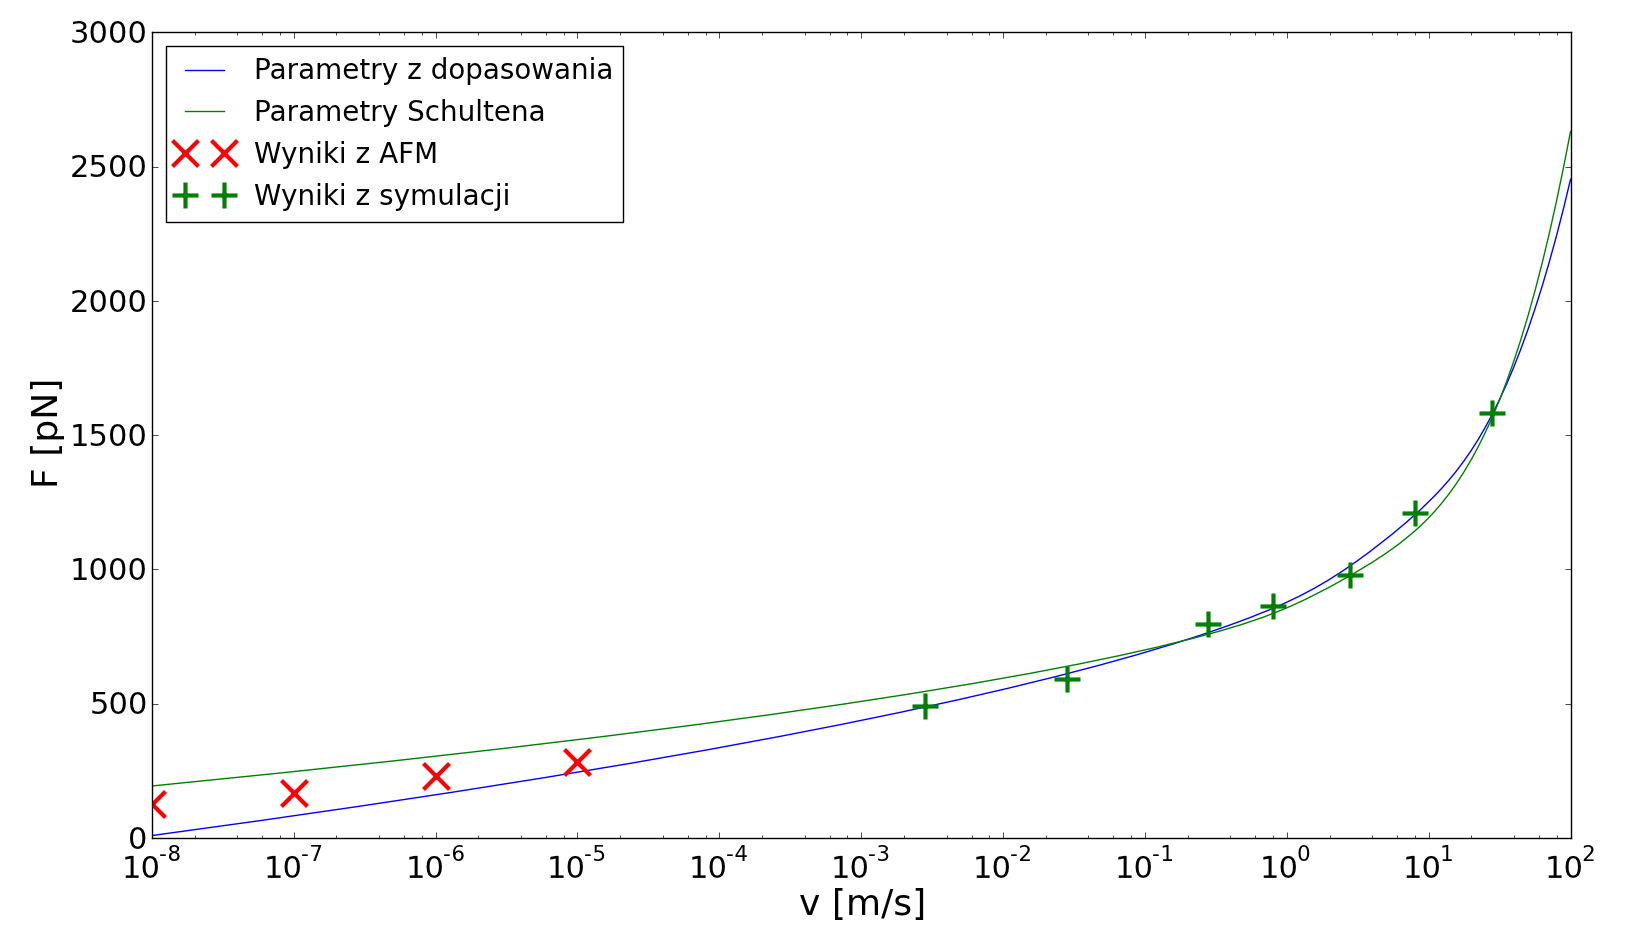
\includegraphics[width=150mm]{./rys/dop_schul.png}
\caption{Wykres krzywej teoretycznej z parametrami z pracy Schultena oraz po dopasowaniu z naniesionymi danymi z eksperymentu AFM.}
\end{centering}
\end{figure}

\begin{table}[H]
\centering
  \begin{tabular}{ l c c c c}
  & F [pN]\\
  \hline
 v [nm/ms]& AFM  & Praca\cite{szul} & Z dopasowania\\
  \hline
0.01 & 125 &  193 & 8.6 \\
0.1 & 166 &  247 & 82 \\
1 & 230 &  304 & 160\\
10 & 283 &  366 & 244\\

\hline
 \hline
  \end{tabular}
  \label{tab1}
  \caption{Przedstawienie sił rozplatania wyliczonych z dopasowania do danych z symulacji w porównaniu do rzeczywistych średnich sił rozplatania zmierzonych w eksperymencie AFM.}
\end{table}

Przy czym zmiana średniej siły zerwania dla v=2.8 m/s z 997 pN na 978 pN czyli o 1.9\% spowodowała zmianę dopasowania $k_0$ o rząd wielkości i zmianę wyznaczanej siły dla prędkości 0.01 nm/ms z 2\e{-2} pN do 8.6 pN.

\section{Analiza wydajności klastra}

Pierwszym etapem w analizie wydajności było zbadanie jakości połączenia realizowanego pomiędzy dwoma komputerami. Komunikacja pomiędzy nimi odbywała się poprzez sieć 1 Gbps, jednak komputery te zostały wyposażone w 2 karty, także teoretyczna przepustowość powinna wynosić 2 Gbps. 

Do analizy wydajności sieci służy narzędzie NetPIPE \cite{netpipe}. 

Analizę przepustowości przeprowadzono zarówno na pojedynczych kartach jak i na obu kartach działających razem.

\begin{center}
\begin{figure}[h]
\begin{centering}
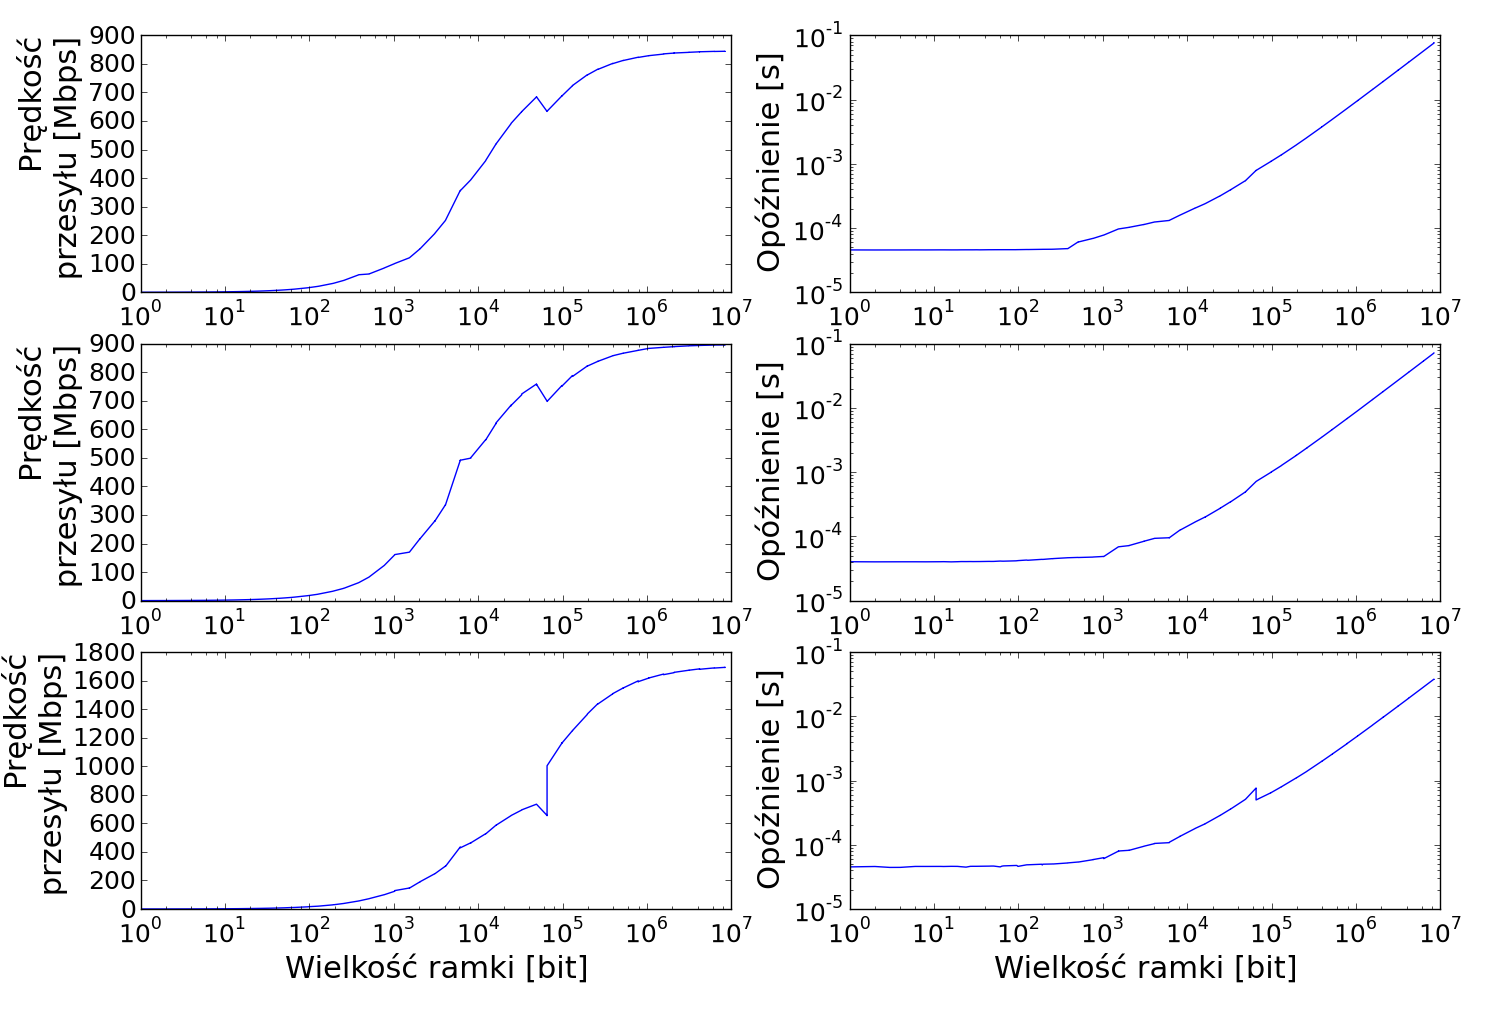
\includegraphics[width=150mm]{./rys/speed.png}
\caption{Wykresy przepustowości oraz opóźnienia dla poszczególnych kart sieciowych oraz dla kart sieciowych działających razem w zależności od wielkości przesyłanych danych.}
\end{centering}
\end{figure}
\end{center}

Na podstawie wykresów można odczytać, że przepustowość komunikacji MPI przez pierwszą jak i przez drugą kartę sieciową wynosi odpowiednio 830 Mbps oraz 890 Mbps. Po włączeniu obu kart sieciowych naraz przepustowość komunikacji rośnie do 1680 Mbps. Opóźnienia dla małych rozmiarów pakietów wynoszą odpowiednio 42 $\mu$s oraz 36 $\mu$s. Dla kart działających razem opóźnienie to wynosi około 45 $\mu$s.

Wyniki te świadczą o wydajnym połączeniu pomiędzy dwoma komputerami, jednak opóźnienia rzędu kilkudziesięciu $\mu$s nijak mają się do tych osiąganych przez sieci typu Infiniband czy też Myrinet, które są o rząd wielkości mniejsze, co pozwala na zmniejszenie opóźnień w komunikacji pomiędzy procesami i w efekcie prowadzi do lepszej skalowalności.

Analiza wydajności klastra polegała na wykonaniu tej samej powtórzonej symulacji na różnej liczby rdzeni, a następnie zbadaniu czasu potrzebnego na obliczenia w zależności od liczby wykorzystywanych rdzeni. Dobrym wyznacznikiem jest liczba ns obliczonych w określonej jednostce czasu, na przykład na dzień. W idealnym przypadku liczba ta powinna rosnąć liniowo wraz ze wzrostem liczby wykorzystywanych rdzeni. 

Do symulacji użyto tego samego układu, który był rozciągany przy prędkości 50~nm/ns. Symulację powtarzano 16 razy idąc od obliczeń na 1 rdzeniu aż do obliczeń na 16 rdzeniach prowadzonych równolegle. Obliczenia te wykonano zarówno z użyciem przydziału osobnych rdzeni na obliczenia PME jak i bez. Powyżej 8 rdzeni komunikacja między komputerami odbywała się poprzez dwie karty 1Gbps. 

Na tej podstawie sporządzono wykresy wydajności liczonych ns/dzień oraz porównano jak obliczona wydajność ma się w stosunku do teoretycznego liniowego wzrostu wydajności. 

\begin{center}
\begin{figure}[h!]
\begin{centering}
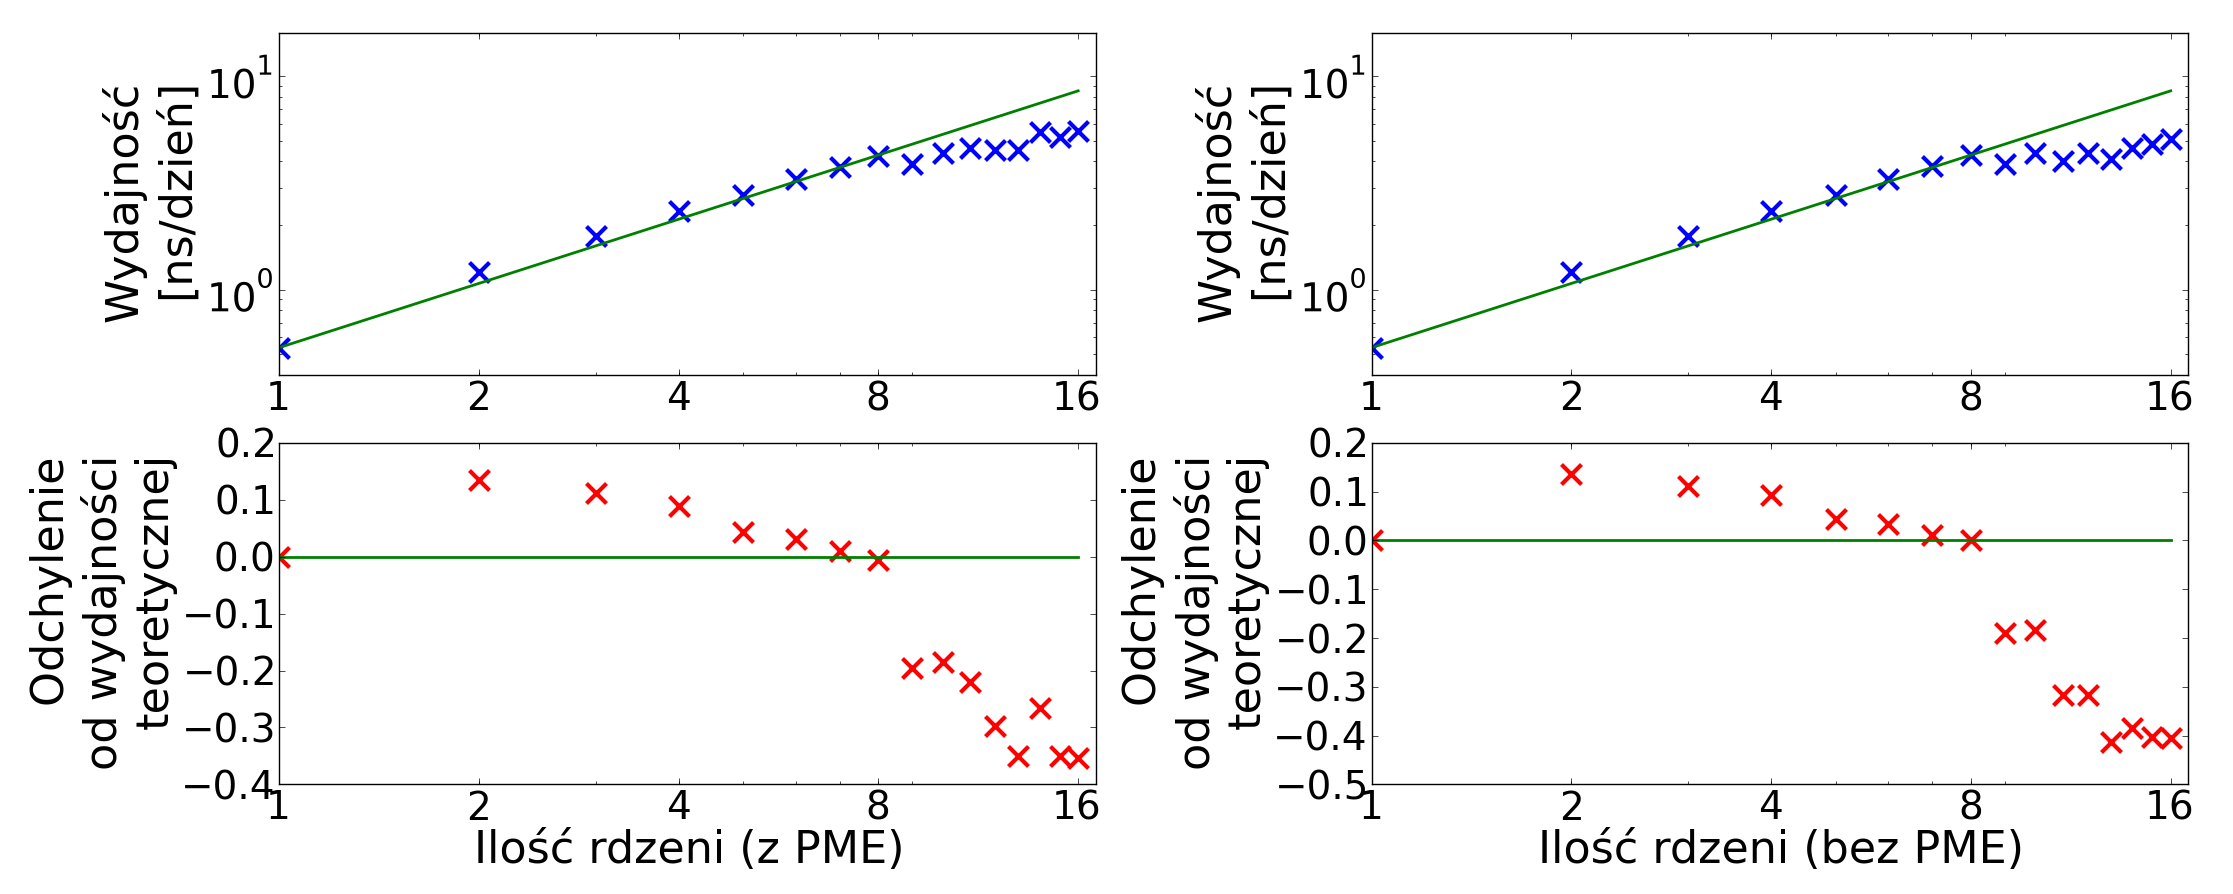
\includegraphics[width=150mm]{./rys/wyd.png}
\caption{Wykres wydajności obliczeń w zależności od liczby użytych rdzeni oraz ich odchyleń od wartości teoretycznych.}
\end{centering}
\end{figure}
\end{center}

Z powyższych wykresów można wnioskować, że skalowalność klastra zachowuje się liniowo aż do bariery 8 rdzeni. Ponadto wydajność obliczeń powyżej 1 rdzenia rośnie powyżej zależności teoretycznej, co świadczy o tym, że obliczenia tylko na jednym rdzeniu są wolniejsze. Po przekroczeniu granicy obliczeń prowadzonych na 8 rdzeniach wydajność w najgorszym przypadku jest o około 40\% mniejsza niż wynikałoby to z linowego wzrostu wydajności. Podobne wyniki dają obliczenia prowadzone przy automatycznym wyborze liczby rdzeni przeznaczonych tylko na obliczenia PME jak i obliczenia prowadzone bez przydziału osobnych rdzeni na obliczenia PME poprzez zastosowanie opcji \texttt{-nopme} w programie \texttt{mdrun}.

Wydajność obliczeń w przypadku zastosowania automatycznego przydziału rdzeni na obliczenia PME jest jednak wyraźnie większa przy wykorzystaniu 16 rdzeni niż bez tego przydziału. 
